\section{Ausdr"ucke und Operatoren}
�hnlich wie mathematische Ausdr�cke stellen auch Ausdr�cke in C++ Berechnungen das und bestehen aus Operanden und Operatoren. Die Auswertung jedes Ausdrucks liefert einen Wert, der sich aus der Verkn�pfung von Operanden durch Operatoren ergibt. 
	\begin{compactitem}
		\item Arithmetische Ausdr�cke: Ausdr�cke, deren Ergebnis als Skalar geschrieben werden kann (char-, int- oder float-Typen). 
		\item Logische Ausdr�cke: Ausdr�cke, die Wahrheitswerte beschreiben. Sie entstehen durch Vergleiche oder logische Verkn�pfungen.
		\item Andere Ausdr�cke: Darunter fallen zum Beispiel Typumwandlungen (Cast-Ausdr�cke) ebenso wie typeid-Ausdr�cke.
	\end{compactitem}
	
	\subsection{Auswertungsreihenfolge}
	Alle Ausdr�cke werden nach bestimmten Regeln ausgewertet. Massgeblich f�r die Art der Auswertung sind dabei Assoziativit�t und Priorit�t der Operatoren. \\\\
	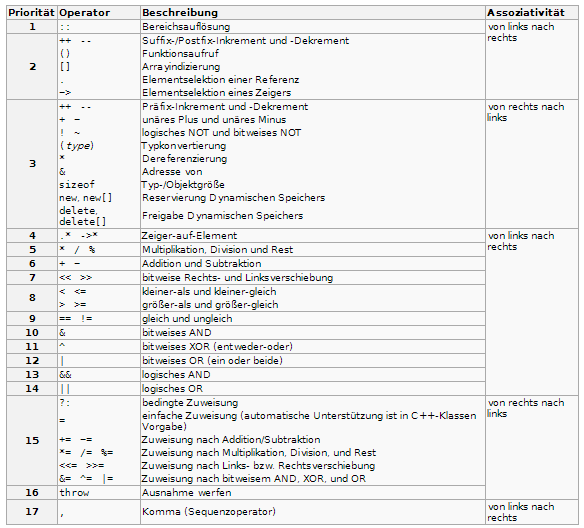
\includegraphics[width=0.6\textwidth]{pics/Priotabelle.png}
	\\(Priorit�t 1 hat Vorrang vor allen anderen)
		\subsubsection{Assoziativit�t}
		Die Assoziativit�t gibt Auskunft �ber die Auswertungsreihenfolge der Operanden eines Ausdrucks. So wird zum Beispiel im Ausdruck p++ zuerst p ausgewertet und dann die linke Seite des Operators ++ (p) erh�ht, w�hrend der Ausdruck ++p zuerst p erh�ht und dann den Ausdruck auswertet.
		\lstinputlisting[language=C++,tabsize=2]{code/prio1.cpp}
		\subsubsection{Priorit�t}
		Die Priorit�t von Operatoren wiederum gibt an, in welcher Reihenfolge die verschiedenen Operanden eines Ausdrucks ausgewertet werden. Die multiplikativen Operatoren weisen zum Beispiel eine h�here Priorit�t als die additiven Operatoren auf.
	\begin{minipage}[t]{13 cm}
	\subsection{L-Werte und R-Werte}
		\begin{compactitem}
			\item Ausdr�cke haben eine unterschiedliche Bedeutung, je nachdem, ob sie links oder rechts vom Zuweisungsoperator stehen.
			\item Ein Ausdruck stellt einen L-Wert (lvalue oder left value) dar, wenn er
			sich auf ein Speicherobjekt bezieht. Ein solcher Ausdruck kann links (und rechts) des Zuweisungsoperators stehen.
			\item Ein Ausdruck, der sich nicht auf ein Speicherobjekt bezieht, kann nur
			rechts des Zuweisungsoperators stehen. Er wird als R-Wert (rvalue oder right value) bezeichnet. Einem R-Wert kann nichts zugewiesen werden.\\
			\lstinputlisting[language=C,tabsize=2]{code/l-r-wert.c}
		\end{compactitem}
	\end{minipage}
	\hspace*{1cm}
	\begin{minipage}[t]{5 cm}
		\vspace*{-0.2cm}
		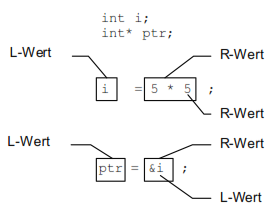
\includegraphics[width=1\textwidth]{pics/l-r-wert1.png}
		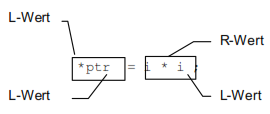
\includegraphics[width=1\textwidth]{pics/l-r-wert2.png}
	\end{minipage}\\
		\subsubsection{Zugriff auf L- und R-Werte}
			\begin{compactitem}
				\item Ein lvalue erfordert immer Schreibzugriff
				\item Auf einen rvalue wird nur lesend zugegriffen
				\item Es gibt auch nicht modifizierbare lvalues. Auf diese kann auch nur lesend zugegriffen werden.
			\end{compactitem}
	 
	\subsection{Operatoren im einzelnen}
		\begin{minipage}[t]{9 cm}
			\subsubsection{Bereichsoperator (Scope Operator) :: }
				Der Bereichs-Operator ist erst in C++ verf�gbar und liefert dem Compiler den Hinweis, in welchem Namespace er nach einem Symbol suchen soll. Der Namespace steht dabei links der beiden Doppelpunkte :: und der Symbolname steht rechts davon.
		\end{minipage}
		\hspace*{0.5cm}
		\begin{minipage}[t]{9 cm}
			\subsubsection{Un�re arithmetische Operatoren}
				\begin{compactitem}
					\item Positiver Vorzeichenoperator $+A$
					\item Negativer Vorzeichenoperator $-A$
					\item Postfix-Inkrementoperator $A++$
					\item Pr�fix-Inkrementoperator $++A$
					\item Postfix-Dekrementoperator $A- -$
					\item Pr�fix-Dekrementoperator $- -A$
				\end{compactitem}
		\end{minipage}
		\\\\
		\begin{minipage}[t]{9 cm}
			\subsubsection{Bin�re arithmetische Operatoren}
				\begin{compactitem}
					\item Additionsoperator $A + B$
					\item Subtraktionsoperator $A - B$
					\item Multiplikationsoperator $A * B$
					\item Divisionsoperator $A / B$
					\item Modulooperator $A \% B$   
				\end{compactitem}	
		\end{minipage}
		\hspace*{0.5cm}
		\begin{minipage}[t]{9 cm}
			\subsubsection{Zuweisungsoperatoren}
				\begin{compactitem}
					\item Zuweisungsoperator $A = B$
					\item Kombinierte Zuweisungsoperatoren
					\begin{compactitem}
						\item Alle arithmetischen und logischen Operatoren haben zusammen mit dem
						Zuweisungsoperator eine verk�rzte Form, die das Schreiben verk�rzt (mehr nicht)
						\item Beispiel:\\
						$a = a / b;$\\
						kann verk�rzt geschrieben werden als\\
						$a /= b;$
					\end{compactitem}
				\end{compactitem}
		\end{minipage}
		\\\\
		\begin{minipage}[t]{9 cm}
			\subsubsection{Relationale Operatoren\newline  (Vergleichsoperatoren)}
				\begin{compactitem}
					\item Gleichheitsoperator $A == B$
					\item Ungleichheitsoperator $A != B$
					\item Gr�sseroperator $A \textgreater \ \ B$
					\item Kleineroperator $A \textless \ \ B$
					\item Gr�ssergleichoperator $A \textgreater= B$
					\item Kleinergleichoperator $A \textless= B$ 
				\end{compactitem}	
		\end{minipage}
		\hspace*{0.5cm}
		\begin{minipage}[t]{9 cm}
			\subsubsection{Logische Operatoren}
				\begin{compactitem}
					\item Logisch UND (AND) $A \&\& B$
					\item Logisch ODER (OR) $A || B$
					\item Logisch NICHT (NOT) $!A$\\\\
					0 = false, falsch\\
					1 = true, wahr (genauer: ungleich 0)
				\end{compactitem}
		\end{minipage}
		\\\\
		\begin{minipage}[t]{9 cm}
			\subsubsection{Bit-Operatoren}
				\begin{compactitem}
					\item Bitweises AND $A \& B$
					\item Bitweises OR $A | B$
					\item Bitweises NOT (Inverter) $\textasciitilde A$
					\item Bitweises XOR $A \wedge B$ 
				\end{compactitem}	
		\end{minipage}	
		\hspace*{0.5cm}	
		\begin{minipage}[t]{9 cm}
			\subsubsection{Schiebe- (Shift-) Operatoren}
				\begin{compactitem}
					\item Rechts-Shift um n Bits $A \textgreater \ \textgreater \ \ n$
					\item Links-Shift um n Bits $A \textless \  \textless \ \ n$
				\end{compactitem}
			\end{minipage}		\\\\					
			\begin{minipage}[t]{9 cm}
				\subsubsection{Bedingungsoperator (Tern�rer Operator)}
					$A ? B : C$\\\\
					Ist eine verk�rzte Schreibweise f�r
					\lstinputlisting[language=C,tabsize=2]{code/Ternaerer_Operator.c}
			\end{minipage}
			\hspace*{0.5cm}
			\begin{minipage}[t]{9 cm}
				\vspace*{0.5cm}
				Beispiel Maximum von zwei Zahlen a, b ermitteln:
				\lstinputlisting[language=C,tabsize=2]{code/Ternaerer_Operator2.c}
				entspricht:
				\lstinputlisting[language=C,tabsize=2]{code/Ternaerer_Operator3.c}	
			\end{minipage}